The tracking systems of ECCE allow for the measurement of lower momentum charged jets with excellent scale and resolution.  The analysis was completed with 18x275 GeV Pythia 8 electron proton collisions, requireing a $Q^2$ greater than $100$ GeV, and the prop.4 detector configuration.  The anti-$k_T$ jet finding algorithm was utilized, with a jet radius $R=0.5$.  To prevent the classification of single particles as jets, a constraint of $z<0.95$ as applied, where 
\begin{equation}
z=\frac{E_{\hbox{most energetic constituent}}}{E_{\hbox{total jet}}}.
\label{eq:jet_z}
\end{equation}

A cut on the transverse momentum of $p_T<30$ was applied to reject higher momentum tracks being reconstructed at lower momentum.  


% Track jet momentum scale and resolution
\todo{regenerate plots as PDF}
\begin{figure}
    \centering
    \begin{subfigure}{0.4\textwidth}
        \centering
        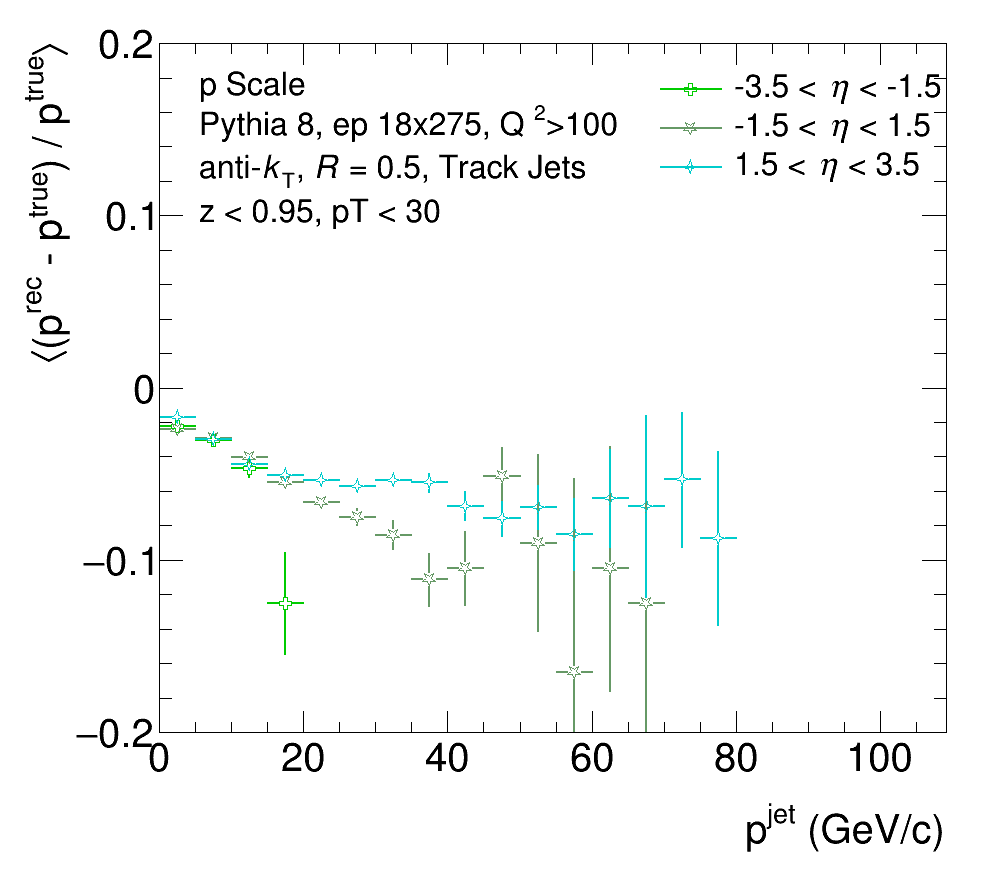
\includegraphics[width=\linewidth]{figs/jet_plots/pScale_track_grouped.png}
        \caption{Track jets scale}
        \label{fig:track_momentum_scale}
    \end{subfigure}
    \hfill
    \begin{subfigure}{0.4\textwidth}
        \centering
        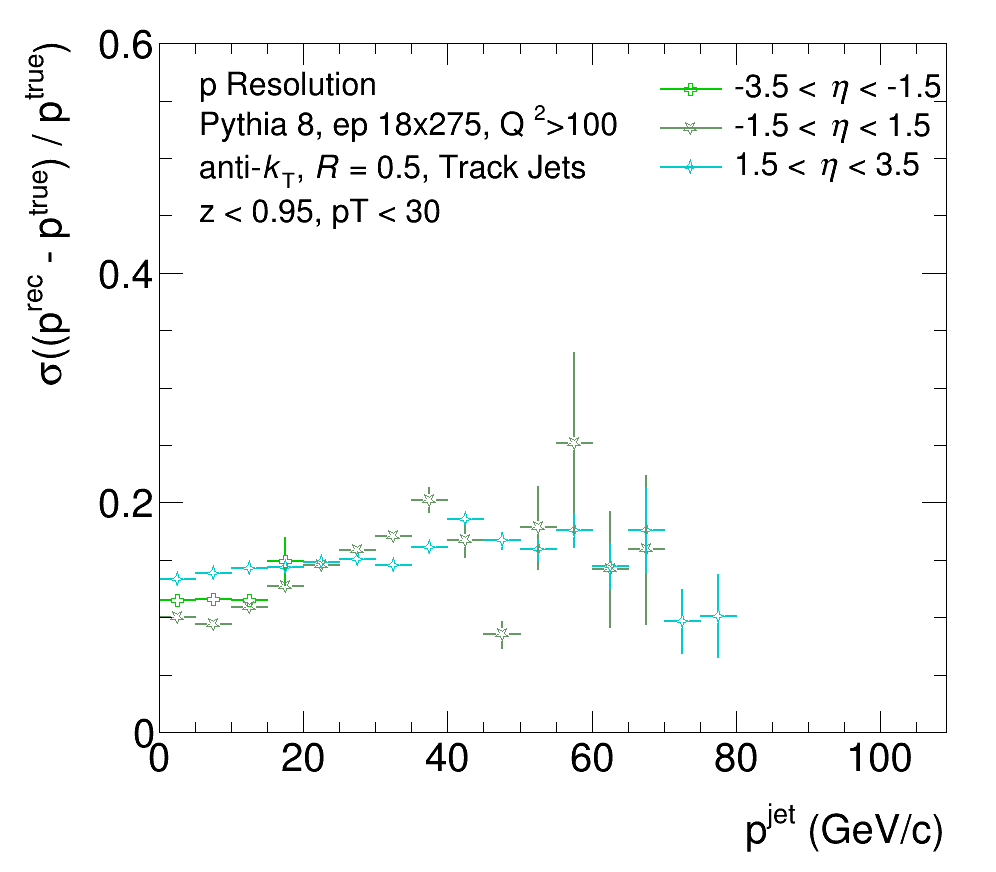
\includegraphics[width=\linewidth]{figs/jet_plots/pReso_track_grouped.png}
        \caption{Track jet resolution}
        \label{fig:track_momentum_resolution}
    \end{subfigure}
    \caption{The scale and resolution of the momentum of track jets.}
    \label{fig:track_momentum_reso_scale}
\end{figure}

As seen in figure \ref{fig:track_momentum_scale}, the scale is better than -0.15 across entire detectors acceptance.  This, in combination with the momentum resolution better than 0.2 as shown in figure \ref{fig:track_momentum_resolution} opens up the ability to study charged jets in great detail, especially in the lower momentum regime.  

% Track jet spatial resolution
\begin{figure}
    \centering
    \begin{subfigure}{0.4\textwidth}
        \centering
        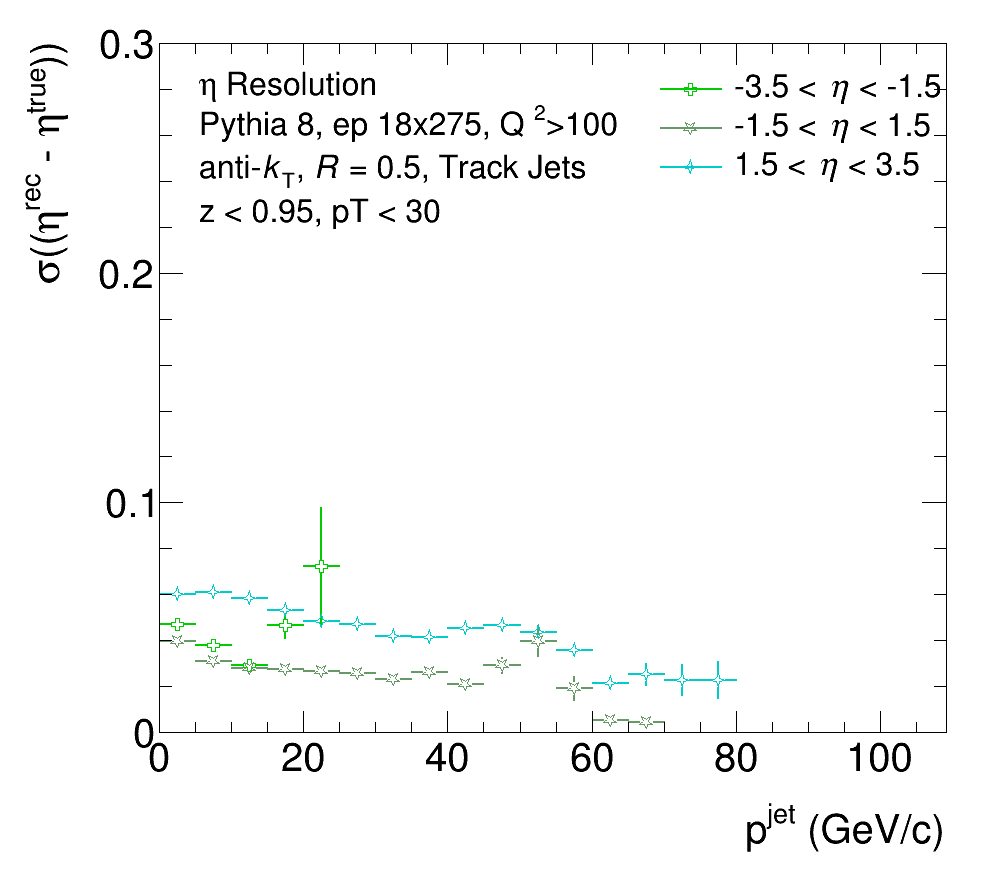
\includegraphics[width=\linewidth]{figs/jet_plots/EtaReso_track_grouped.png}
        \caption{Track jet $\eta$ resolution}
        \label{fig:track_eta_resolution}
    \end{subfigure}
    \hfill
    \begin{subfigure}{0.4\textwidth}
        \centering
        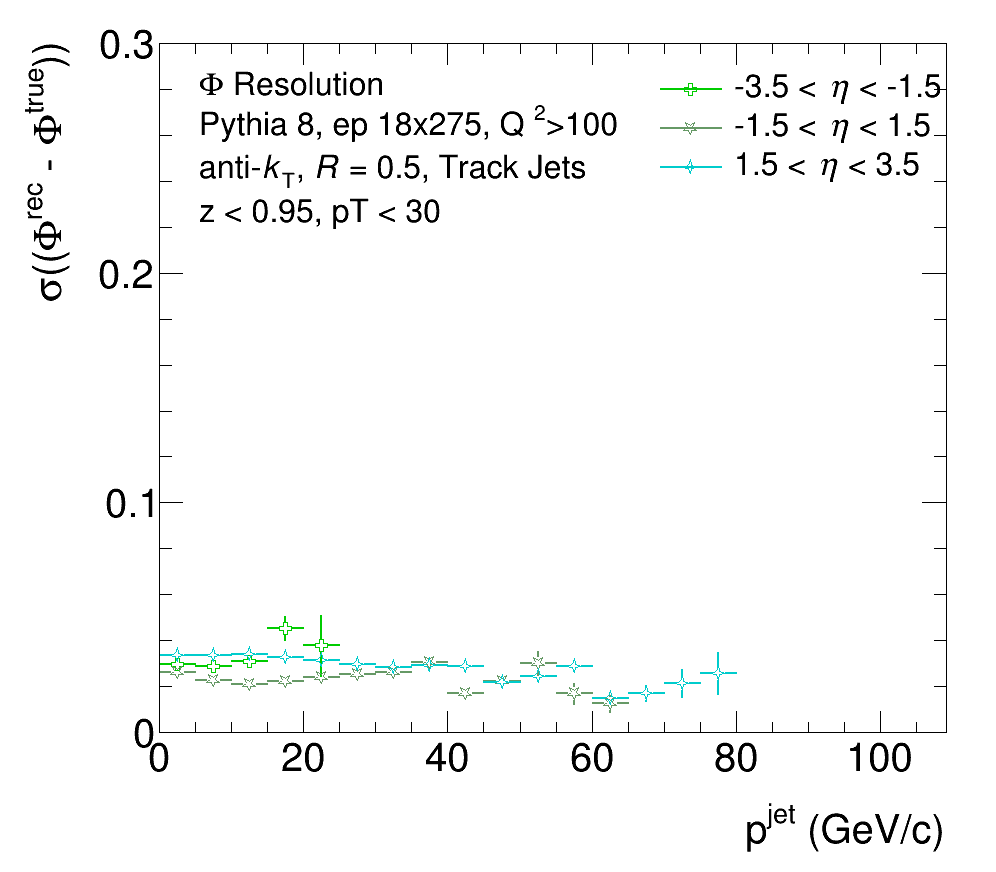
\includegraphics[width=\linewidth]{figs/jet_plots/PhiReso_track_grouped.png}
        \caption{Track jet $\phi$ resolution}
        \label{fig:track_phi_resolution}
    \end{subfigure}
    \caption{The spatial resolution of track jets}
    \label{fig:track_spatial_reso_scale}
\end{figure}

In addition to the excellent momentum scale and resolution the ECCE tracking system offers, the detector offers very good spatial resolution of jets (Figure \ref{fig:track_spatial_reso_scale}).  